\chapter*{Flags d'optimisation}

On a éssayé différents flags de compilation suivant le processeur.

\section*{Pour gcc}
\begin{itemize}
    \item{-Og: n'active que les optimisations triviales. Nous avons choisi de tester ce flag uniqument pour voir si les optimisations avait un quelconque effet}
    \item{-O3: référence, nous avons pu voir avec maqao que la puissance processeur reste mal exploité notament à cause du manque de vectorisation, option pourtant activé.}
    \item{-Ofast: Optimisation agressive, violation de certains standards IEEE. Ce flag devrait permettre d'accélérer la division présente }
    \item{-funsafe-math-optimizations : compris dans -Ofast, IEEE non-strict. Ce flag est compris dans Ofast nous l'avons tester à part pour voir si la totalité de Ofast était utile } 
    \item{-ffast-math: Flottants non associatifs + IEEE non stricts.}
    \item{-frename-registers: technique de renommage de registres, pour éliminer certaines dépendances inter-instructions}
    \item{-fsection-anchors: Optimisation agressive sur les accés mémoire pour diminuer le calcul d'adresse-non disponble sur l'architecture cible}
\end{itemize}

\section*{Pour icc}
\begin{itemize}
    \item{-O3 niveau d'optimisation équivalent à celui de gcc}
    \item{-fast : optimistation ultra agressive, qui donne un code très rapide, mais il nous était impossible de l'anaylser avec maqao. Quelques doutes subsistaient sur sa consistance, avant l'examen du listing assembleur}
    \item {-Ofast: similaire à gcc}
\end{itemize}   

\section*{Comparaisons}

\subsection*{Temps en L1}
\begin{figure}[ht!]
\centering
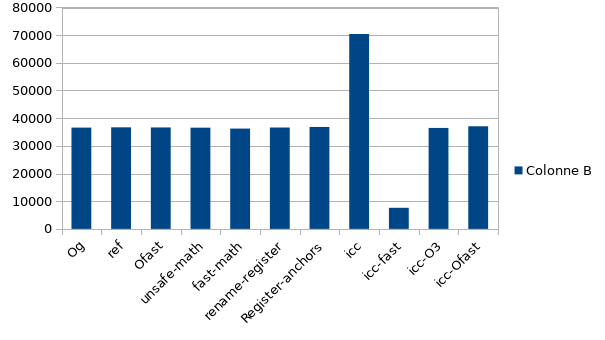
\includegraphics[width=120mm]{MEDIA/time_L1.png}
\caption{Temps selon les flags utilisés en L1}
\end{figure}
On remarque que icc avec le flag fast, génère un code bien plus rapide que gcc.
Cela vient du fait que bien qu'elle soit activée, gcc ne vectorise pas le code.\\
Comme dit plus haut nous n'avons pas pu faire l'analyse du binaire généré avec icc -fast avec maqao. En effet les résultats de maqao fournis n'étaitent pas cohérents
 ( nombre de boucles différent entre 2 expériences sur un binaire identitique, instructions non reconnues, etc ). Nous avons donc décidé d'eximiner le listing assembleur produit pour le kernel,\\
 avec icc sans flag ( autre que -S pour obtenir le listing ) et icc -fast. La première différence est la zone des ".byte" ne connaissant pas assez bien l'assembleur nous ne savons pas à quoi cette zone servait.
La deuxième est qu'une bonne partie des instructions scalaires ont été remplacées par des instructions vectorielles AVX
( movss -> vmovss, divss -> vdivss ). On peut aussi observer que la double boucle a été deroulée, ce qui est déjà le cas sans flag. Nous avons aussi regardé le listing généré pour gcc en O3 ce qui nous a bien confirmé qu'aucune vectorisation n'a été appliquée.
\newpage
\subsection*{Temps en L2}
\begin{figure}[ht!]
    \centering
    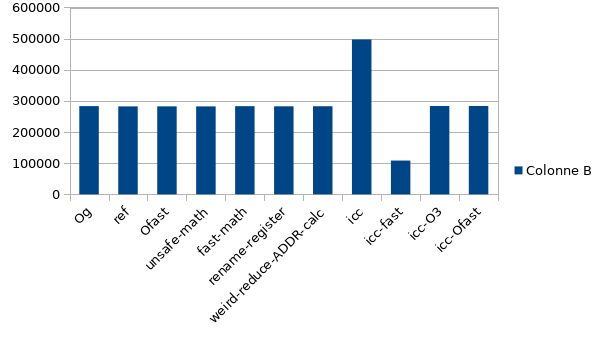
\includegraphics[width=120mm]{MEDIA/Resultat_TEST_L2.png}
    \caption{Temps selon les flags utilisés en L2}
\end{figure}
\subsection*{Temps en L3}
\begin{figure}[ht!]
    \centering
    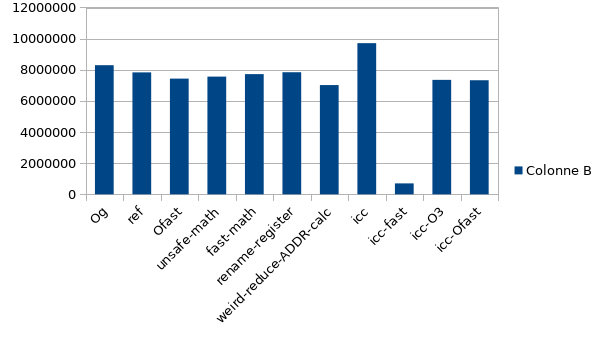
\includegraphics[width=120mm]{MEDIA/Resultat_TEST_L3.png}
    \caption{Temps selon les flags utilisés en L3}
\end{figure}
